\section*{Dati e risultati}

\subsection{Rilevatore di picchi}

In questa sezione ci occuperemo di verificare il corretto funzionamento di un circuito rilevatore di picchi costruito con un diodo 1N4007. Il circuito che abbiamo utilizzato è schematizzato in Figura \ref{fig:circuito_peak}.
In questa configurazione abbiamo impostato che il valore di capacità ($C$) fosse di $1\,\si{\micro\farad}$, mentre il valore della resistenza $R_2$ fosse di $1\,\si{\kilo\ohm}$. Ricordiamo che sul valore della capacità abbiamo un incertezza nominale dell'$1\,\%$,mentre sulla resistenza vi è un errore nominale del $5\,\%$.
Il circuito è stato alimentato con una differenza di potenziale pico-pico in entrata di $10\,\si{\volt}$ ad una frequenza di $100\,\si{\hertz}$.
Quindi per verificare il corretto funzionamento del nostro rilevatore di picchi visuaizziamo la tensione in uscita ($V\ped{out}$) e ne studiamo l'andamento al variare di $C$ e della resistenza $R_1$.
Aggiungiamo che per semplificare le operazioni abbiamo deciso di variare la resistenza $R_1$ mantenedocostante la capacità, e di variare $C$ mantenendo costante $R_2$.
Di seguito riportiamo gli andamenti della tensione in uscita ($V\ped{out}$) al variare di $C$ e di $R_1$.

\begin{SCfigure}
    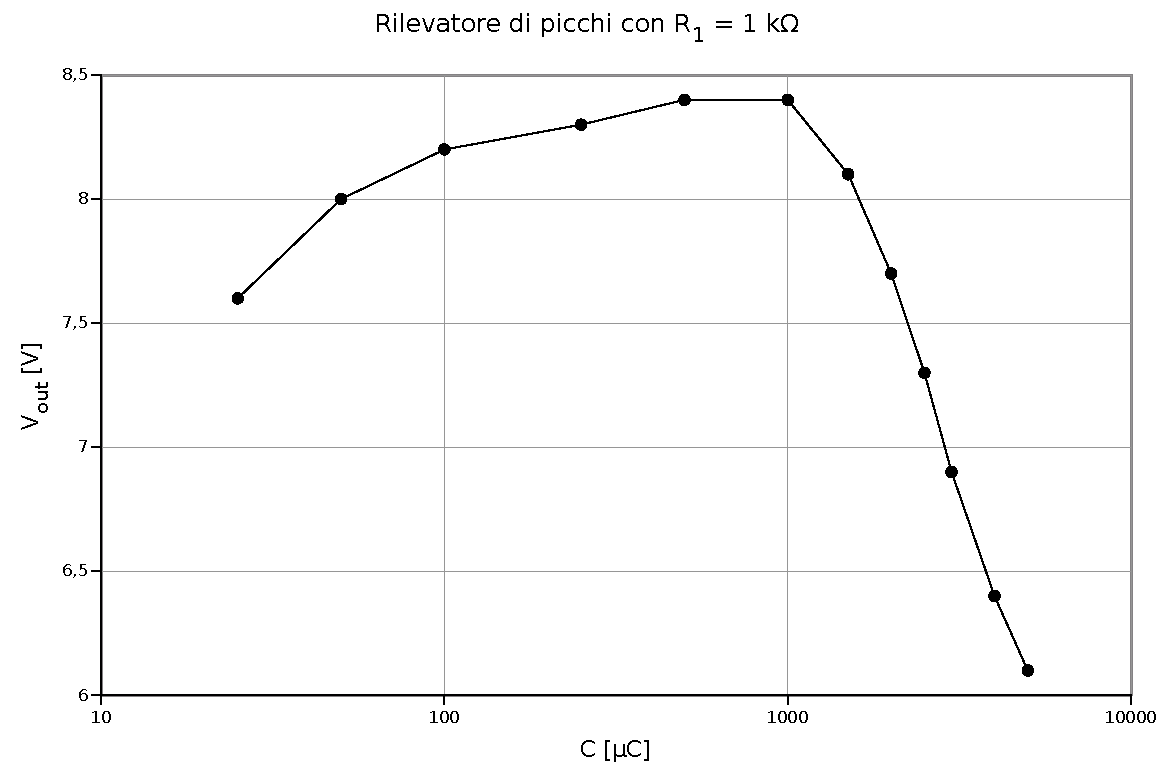
\includegraphics[scale=0.7]{capacita.pdf}
    \caption{}
    \label{fig:capacita}
\end{SCfigure}

\begin{SCfigure}
    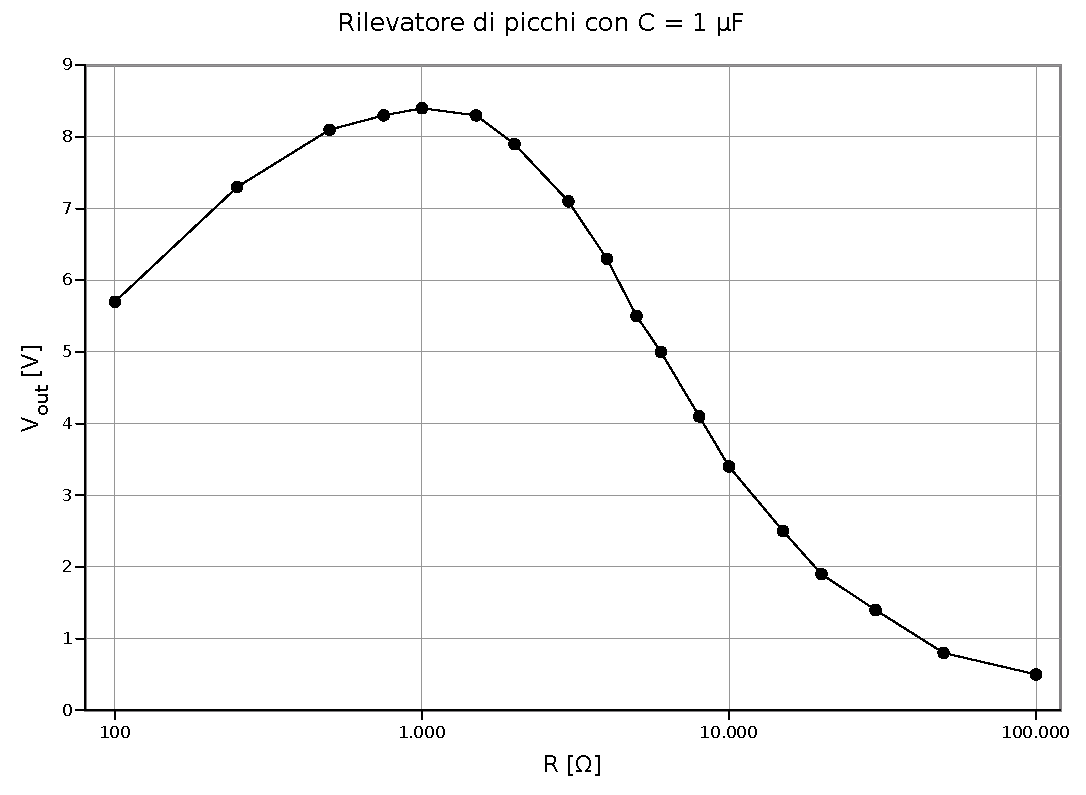
\includegraphics[scale=0.7]{resistenza.pdf}
    \caption{Andrea è un party dancer. Sono un fucking spammer.}
    \label{fig:resistenza}
\end{SCfigure}

Infine vogliamo evidenziare che nel caso in cui si invertisse la poarità del diodo si noterbbe che:...

\subsection{Diodo Zener}

In questa seconda sezione vogliamo studiare la caratteristica $I-V$ in polarizzazione inversa de

\begin{SCfigure}
    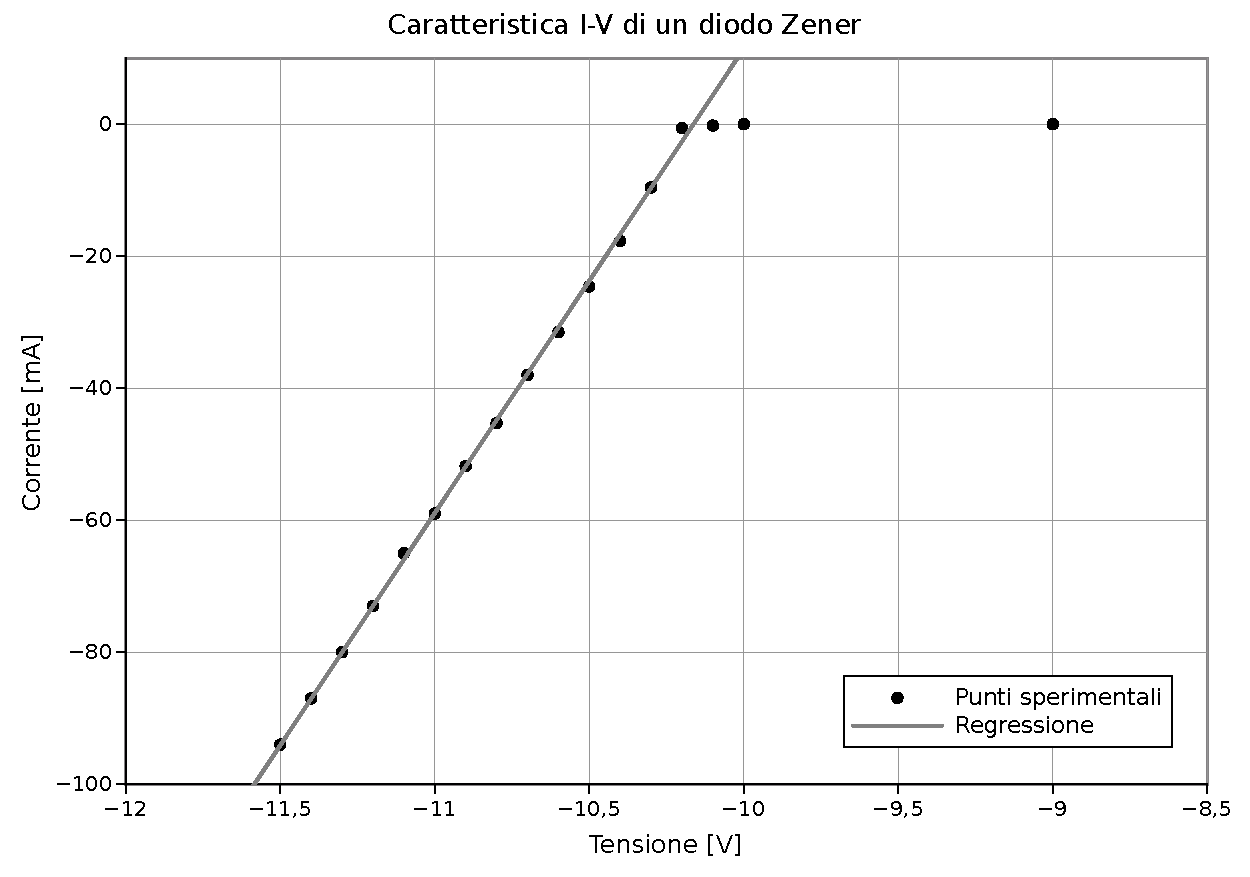
\includegraphics[scale=0.7]{cara_zener.pdf}
    \caption{Andrea è un party dancer. Sono un fucking spammer.}
    \label{fig:resistenza}
\end{SCfigure}

\begin{SCfigure}
    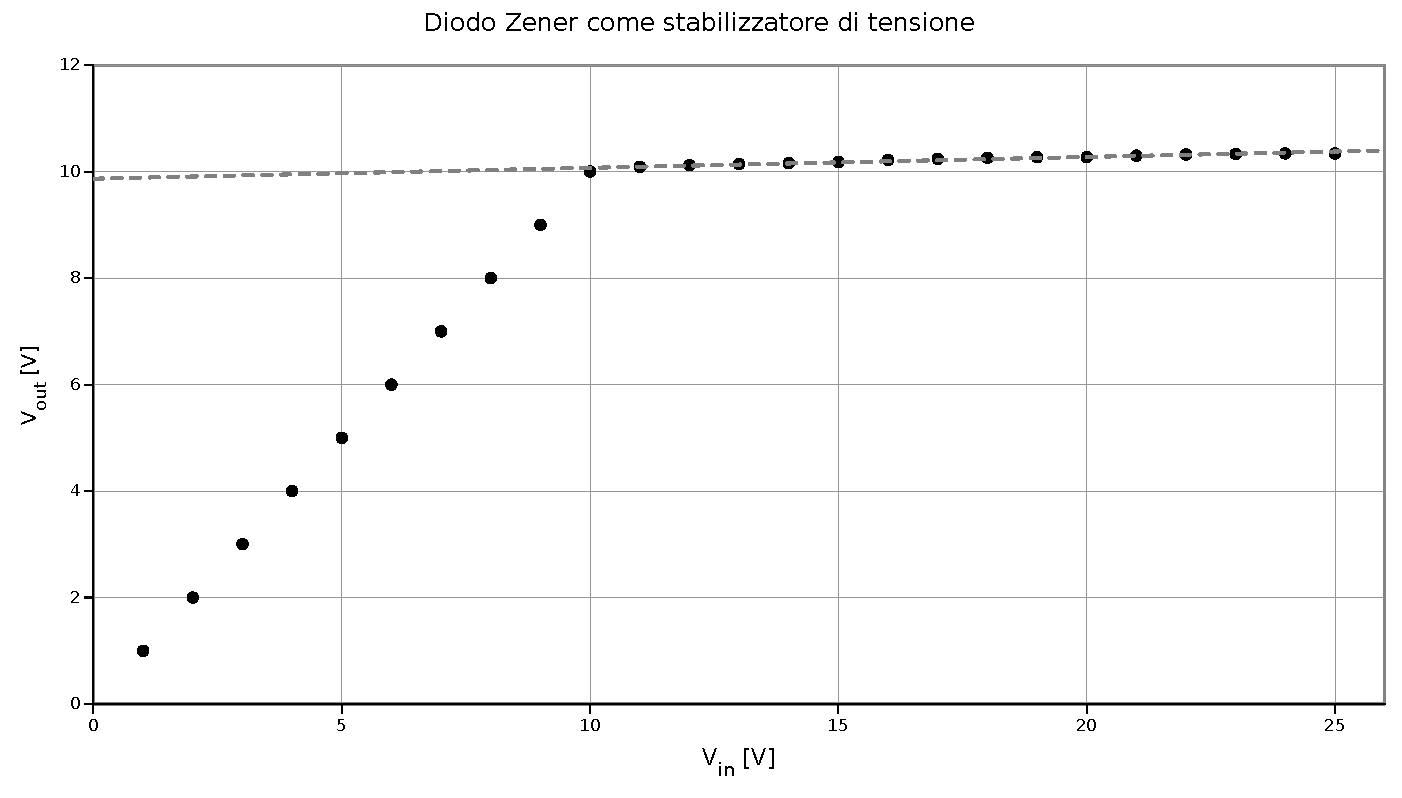
\includegraphics[scale=0.7]{stab.pdf}
    \caption{Andrea è un party dancer. Sono un fucking spammer.}
    \label{fig:resistenza}
\end{SCfigure}
